%% INFS4205/7205 Assignment 3 — Personalised Multimodal Recipe Agent
%% Rename this file before submission: <StudentID>_<Name>.tex
%% Compile: pdflatex report.tex (twice for cross-refs)
%% Requires: acmart.cls (download from https://www.acm.org/publications/proceedings-template)

\documentclass[sigconf, nonacm=true, anonymous=false]{acmart}
\settopmatter{printacmref=false, printccs=false, printfolios=true}
\pagestyle{plain}
\acmConference[INFS4205/7205]{Assignment 3 — Multimodal Agents}{2026}{The University of Queensland}

\usepackage{graphicx}
\usepackage{booktabs}
\usepackage{array}             % for >{\raggedright\arraybackslash}p{} columns
\usepackage{tikz}
\usetikzlibrary{positioning, arrows.meta}

\begin{document}

\title{Personalised Multimodal Recipe Agent:\\
A Component-Level Comparison from Plain LLM to LangGraph}

\author{Yutong Wu}
\affiliation{%
  \institution{School of EECS, The University of Queensland}
  \city{Brisbane}\country{Australia}}
\email{s47790726@student.uq.edu.au}

\begin{abstract}
We build a personalised recipe-QA testbed and use it to quantify the
\emph{marginal} contribution of each component in a typical multimodal
agent stack. Four progressively more sophisticated systems (V0 plain LLM,
V1 text RAG, V2 multimodal RAG, V3 LangGraph agent) and three V3 ablations
(no-memory, no-planner, no-verifier) are evaluated over 20 queries spanning
factual, cross-modal, multi-hop, and conversational families, with
fully programmatic rule-based scoring against a 20-recipe knowledge base.
Retrieval, multimodal fusion, memory, and verification are each shown to
contribute positively. However, we identify a \emph{negative} marginal
benefit of structured planning on multi-hop and conversational queries:
removing the planner from V3 raises overall task success from 65\% to 75\%,
at $\sim$3.6$\times$ the token cost. The result challenges the assumption
that more architecture is monotonically better and supports a
query-type-dependent design.
\end{abstract}

\maketitle

% =====================================================================
\section{Introduction}
\label{sec:intro}

Retrieval-Augmented Generation (RAG) and agent frameworks such as
LangGraph have made it tractable to build multimodal QA systems that
combine retrieval, planning, tool use, and memory. A common assumption is
that each added layer of complexity yields a monotonic improvement in
answer quality. However, the \emph{component-level marginal benefit} of
each layer is rarely measured directly: most published systems report a
single end-to-end number against a baseline without isolating which
component carries the gain.

We frame this work as a systems study rather than a system proposal.
Specifically, we ask:
\emph{retrieval} aside, do \emph{multimodal} indices, \emph{persistent
memory}, \emph{explicit planning}, and \emph{constraint verification}
each contribute positive marginal value, and on which query types?

\smallskip\noindent\textbf{Contributions.}
\begin{itemize}\setlength\itemsep{1pt}
  \item A controlled comparison of 7 system configurations (4 progressive
        baselines plus 3 V3 ablations) on the same 20-query test set,
        with the underlying LLM held constant.
  \item A 20-recipe personalised knowledge base co-designed with the test
        queries to enable \emph{purely rule-based} evaluation, with
        verifiable constraints replacing LLM-as-judge.
  \item A 5-class failure taxonomy aligned with the RAG Triad
        \cite{rag-triad}, separating retrieval, grounding, reasoning,
        query-grounding, and citation failures.
  \item A counter-intuitive finding: \textbf{structured planning has
        negative marginal benefit on multi-hop and conversational
        queries}, suggesting that explicit plans can be more brittle than
        reactive tool calling when query semantics are ambiguous.
\end{itemize}

% =====================================================================
\section{Personalised Knowledge Base}
\label{sec:kb}

The knowledge base contains 20 recipes (\texttt{data/recipes.json}) with
paired AI-generated photographs (\texttt{images/}). Each recipe carries
structured fields: cuisine, prep / cook / total minutes, servings, main
protein, ingredients (name, amount, unit), dietary tags, allergens,
cooking methods, step list, an image caption, and a
\emph{visual attributes} block (dominant colours, presentation,
visible ingredients).

The recipe set is intentionally curated so that gold answers are
computable from the structured fields, not opinion-based:
\begin{itemize}\setlength\itemsep{1pt}
  \item Three recipes containing \emph{eggs, tomato, and onion}
        (cook times 8 / 30 / 40 min), enabling a deterministic
        \texttt{argmin} test (QF3.1).
  \item Exactly two recipes containing both garlic \emph{and} ginger
        (QF3.3 set-intersection test).
  \item Three Thai dishes, two with peanuts and one without (QF4.1
        allergen test).
  \item Visually similar but cuisine-distinct distractor pairs
        (tonkatsu / tempura / fried\_chicken; curry-udon / pad-thai)
        used in adversarial cross-modal probes (QF2.4, QF2.5).
  \item A vegan recipe with the shortest prep time (avocado-toast, 2~min;
        QF3.2 superlative test).
\end{itemize}
This adversarial co-design lets us check answers programmatically against
hard facts, eliminating self-evaluation bias.

% =====================================================================
\section{Retrieval Design}
\label{sec:retrieval}

Both text and images are encoded into a shared joint space using
\emph{OpenCLIP} ViT-B-32 \cite{openclip} (LAION-2B pretrained weights). Two ChromaDB \cite{chromadb} collections are persisted
under \texttt{chroma\_db/}: \texttt{recipes\_text}, where the document
per recipe concatenates name, cuisine, ingredients, methods, dietary
tags, and image caption; and \texttt{recipes\_image}, where each
document is the CLIP image embedding of the recipe photograph.

We use \emph{two separate indices} rather than a single fused index
deliberately: this lets the V3 planner choose between modalities (and
lets us ablate that choice). V2 always queries both indices and merges
candidates by interleaved rank, deliberately exercising the
``always-fuse'' opposite of V3's routing.

% =====================================================================
\section{Agent Workflow}
\label{sec:agent}

\textbf{V0--V2 baselines.} V0 is a plain LLM call. V1 retrieves top-3
text candidates and passes them as context. V2 retrieves top-3 from both
text and image indices, fuses them by interleaved rank, and passes the
union (up to 5) as context. No memory, no tools.

\textbf{V3 (full agent).} A LangGraph \cite{langgraph} state machine
with six nodes and five tools (Figure~\ref{fig:v3arch}). The planner
produces a structured JSON plan over the five tools; the executor
runs each step with
\texttt{\$step\_N} reference resolution; the verifier re-extracts hard
constraints from query + memory and filters candidates accordingly; the
generator writes the final answer; \texttt{memory\_update} extracts
durable facts (allergies, dislikes, cooked-yesterday) from the user's
latest message and persists them.

\textbf{Single-LLM principle.} Every LLM call across V0--V3 (planner,
verifier, generator, memory\_update, V0/V1/V2 single-shot) uses the same
DeepSeek V4 Flash \cite{deepseek} instance via the OpenAI-compatible API
at temperature $0$. This isolates architectural choices as the only
variable between systems.

\textbf{Ablations.} Three V3 configurations disable one node group each:
\textsc{V3-no-memory} skips \texttt{memory\_load} and
\texttt{memory\_update}; \textsc{V3-no-planner} replaces the
planner+executor with a reactive \texttt{bind\_tools} loop where the LLM
decides tool calls iteratively (capped at 6 rounds); \textsc{V3-no-verifier}
passes executor results directly to the generator.

\begin{figure}[t]
\centering
\resizebox{\columnwidth}{!}{%
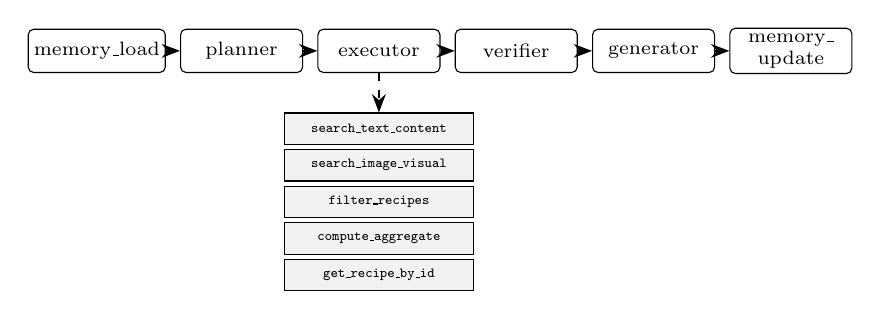
\begin{tikzpicture}[
    node distance=0.35cm and 0.18cm,
    box/.style={draw, rectangle, rounded corners=2pt,
                minimum height=0.55cm, minimum width=1.55cm,
                font=\scriptsize, align=center, inner sep=2pt},
    tool/.style={draw, rectangle, fill=gray!10,
                 minimum height=0.4cm, minimum width=2.4cm,
                 font=\tiny\ttfamily, inner sep=1pt},
    arrow/.style={->, >=Stealth, thick}]
  \node[box] (ml) {memory\_load};
  \node[box, right=of ml] (pl) {planner};
  \node[box, right=of pl] (ex) {executor};
  \node[box, right=of ex] (vf) {verifier};
  \node[box, right=of vf] (gn) {generator};
  \node[box, right=of gn] (mu) {memory\_\\update};
  \draw[arrow] (ml) -- (pl);
  \draw[arrow] (pl) -- (ex);
  \draw[arrow] (ex) -- (vf);
  \draw[arrow] (vf) -- (gn);
  \draw[arrow] (gn) -- (mu);

  \node[tool, below=0.5cm of ex] (t1) {search\_text\_content};
  \node[tool, below=0.05cm of t1] (t2) {search\_image\_visual};
  \node[tool, below=0.05cm of t2] (t3) {filter\_recipes};
  \node[tool, below=0.05cm of t3] (t4) {compute\_aggregate};
  \node[tool, below=0.05cm of t4] (t5) {get\_recipe\_by\_id};
  \draw[arrow, dashed] (ex.south) -- (t1.north);
\end{tikzpicture}}
\caption{V3 agent. Six LangGraph nodes operate over a shared state;
the executor dispatches to five callable tools. Ablations disable
\texttt{memory\_*} (no-memory), \texttt{verifier} (no-verifier), or
replace \texttt{planner+executor} with reactive \texttt{bind\_tools}
(no-planner).}
\label{fig:v3arch}
\end{figure}

% =====================================================================
\section{Experimental Setup}
\label{sec:setup}

\textbf{Query set.} 20 queries are split equally across four families
(5 each): \textbf{factual} (single-fact look-up, plus QF1.5 as an
out-of-KB hallucination probe), \textbf{cross-modal} (visual property
queries, including two adversarial cuisine-exclusion probes),
\textbf{multi-hop} (filter-then-aggregate, set intersection,
multi-constraint), and \textbf{conversational} (2--3 turn scripts testing
allergen accumulation, negative recall, preference conflict, and
constraint override).

\textbf{Constraints.} Each query carries one or more verifiable
constraints drawn from 11 deterministic check types
(\textit{contains-number}, \textit{mentions-recipe}, \textit{does-not-mention},
\textit{subset-of}, \textit{recipe-count}, \textit{indicates-no-recipe},
\textit{identifies-superlative}, \textit{acknowledges-conflict}, etc.).
\emph{Task success} is 1 iff all constraints for the query pass.

\textbf{Metrics.} We report Recall@3 against gold recipe IDs (skipped
when the query is out-of-KB or aggregate-valued); task success;
faithfulness (numeric- and name-claim support against retrieved
context); visual grounding (cross-modal only; colour and presentation
words checked against \emph{visual attributes}); and three efficiency
metrics (end-to-end latency, tool calls, and input+output tokens).

\textbf{Memory contract.} Memory is reset between test cases, not
between turns within a multi-turn case, ensuring within-conversation
context for V3 but no leakage between independent queries.

\textbf{Caching and reliability.} Each \texttt{(system, query)} record is
cached after a fully successful run; failed records are logged and never
written to cache, so re-runs retry only failed pairs. The LLM wrapper
retries 429/5xx errors with exponential backoff (max 3 attempts) and
otherwise raises to the outer loop. All 140 records succeeded in the
final run reported here.

% =====================================================================
\section{Results}
\label{sec:results}

\subsection{Overall task success}

Table~\ref{tab:taskmatrix} and Figure~\ref{fig:heatmap} show task
success per (system, family). The headline pattern is that
\emph{complexity is not monotonically beneficial}: while V0$\to$V1$\to$V2
shows progressive gains, the move from V2 to the full V3 agent
\emph{loses} 0.2 absolute points on multi-hop and conversational. The
best overall system is in fact V3-no-planner (15/20 = 0.75), revealing
that V3's structured planner is a net cost on the two hardest families.

\begin{table}[t]
\centering\small
\caption{Task success per system $\times$ query family ($n=5$ each).
Overall = unweighted mean of the four families.}
\label{tab:taskmatrix}
\begin{tabular}{lccccc}
\toprule
System & Fact. & X-mod. & M.-hop & Conv. & \textbf{Overall} \\
\midrule
V0              & 0.60 & 0.60 & 0.00 & 0.00 & 0.30 \\
V1              & 1.00 & 1.00 & 0.20 & 0.00 & 0.55 \\
V2              & 0.80 & 1.00 & 0.60 & 0.40 & 0.70 \\
V3 (full)       & 1.00 & 1.00 & 0.40 & 0.20 & 0.65 \\
\midrule
V3-no-memory    & 1.00 & 0.80 & 0.60 & 0.00 & 0.60 \\
V3-no-planner   & 1.00 & 0.80 & 0.60 & \textbf{0.60} & \textbf{0.75} \\
V3-no-verifier  & 1.00 & 0.80 & 0.20 & 0.40 & 0.60 \\
\bottomrule
\end{tabular}
\end{table}

\begin{figure}[t]
\centering
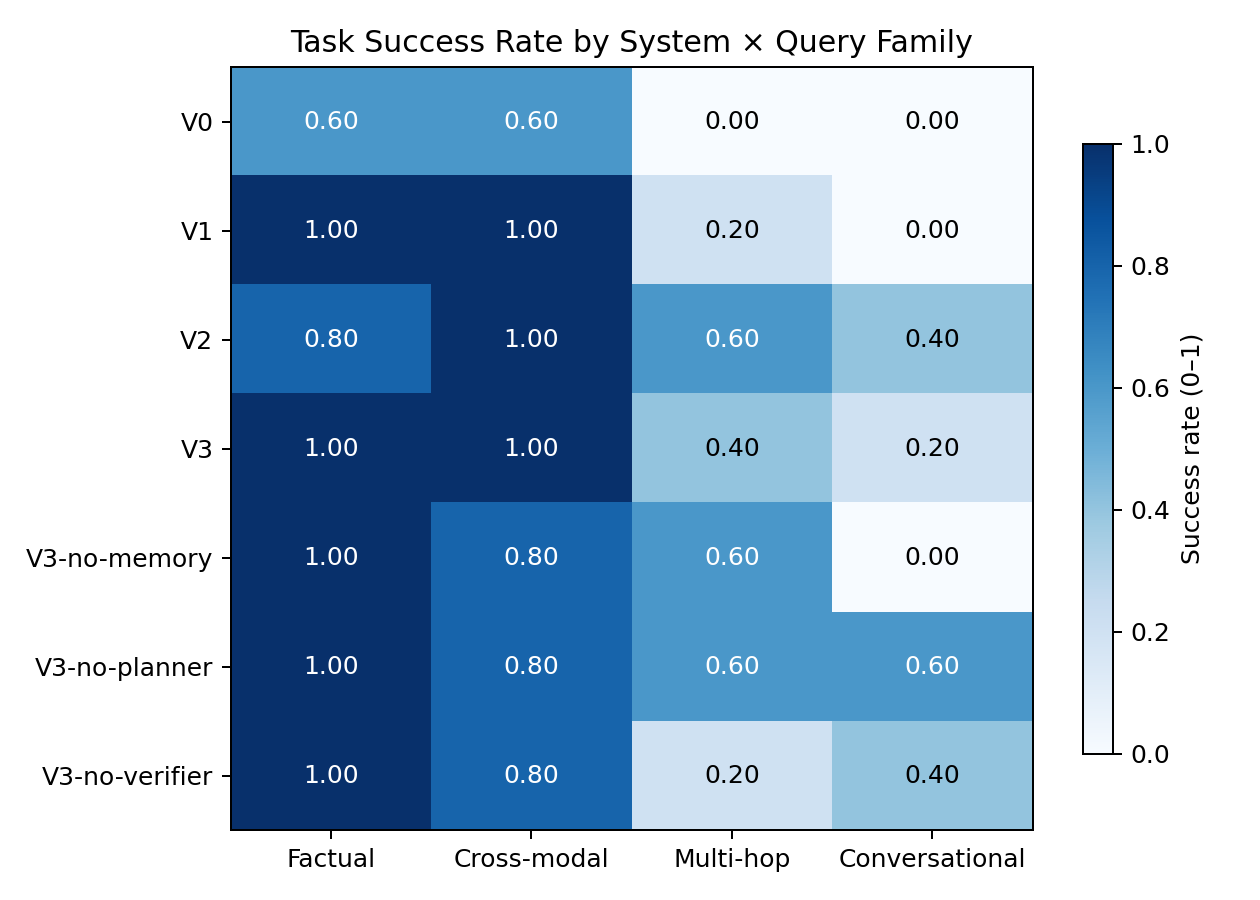
\includegraphics[width=\columnwidth]{eval/results/figures/task_success_heatmap.png}
\caption{Task success heatmap across all seven configurations and four
query families. Darker is better.}
\label{fig:heatmap}
\end{figure}

\subsection{Where each component contributes positively}

\textbf{Retrieval is decisive.} Adding a single text index (V0$\to$V1)
raises faithfulness from 0.00 to 1.00 on every family and lifts
factual+cross-modal task success from 0.6 to 1.0. V0's answers on
multi-hop and conversational queries are 0\% successful: without
retrieval the LLM cannot select among private recipes and either
hallucinates (QF1.5) or politely defers (most of QF3, QF4).

\textbf{Multimodal fusion helps multi-hop.} V1$\to$V2 lifts multi-hop
from 0.20 to 0.60 (e.g. V2 newly passes QF3.1, QF3.2, QF3.5) by
broadening retrieval through the image index --- the image index
sometimes surfaces candidates the text index misses for
ingredient-combination queries.

\textbf{Memory is essential for conversational.} V3-no-memory scores
0/5 on conversational, identical to V0 and V1 on that family. The
allergen-accumulation case (QF4.1) and the preference-conflict case
(QF4.4) both depend on facts surfaced in turn~1 being applied in
turn~2; without persistent memory there is no mechanism for this.

\textbf{Verifier improves cross-modal grounding.} V3 attains a visual
grounding score of 0.93 (cross-modal queries only), versus 0.82 for
V2 and 0.85 for V1: the verifier filters out candidates whose
\emph{visual attributes} do not match the query's colour or
presentation descriptors, raising the share of grounded descriptors
in the final answer.

\subsection{When planning hurts: a negative marginal benefit}
\label{sec:planner-neg}

\begin{figure}[t]
\centering
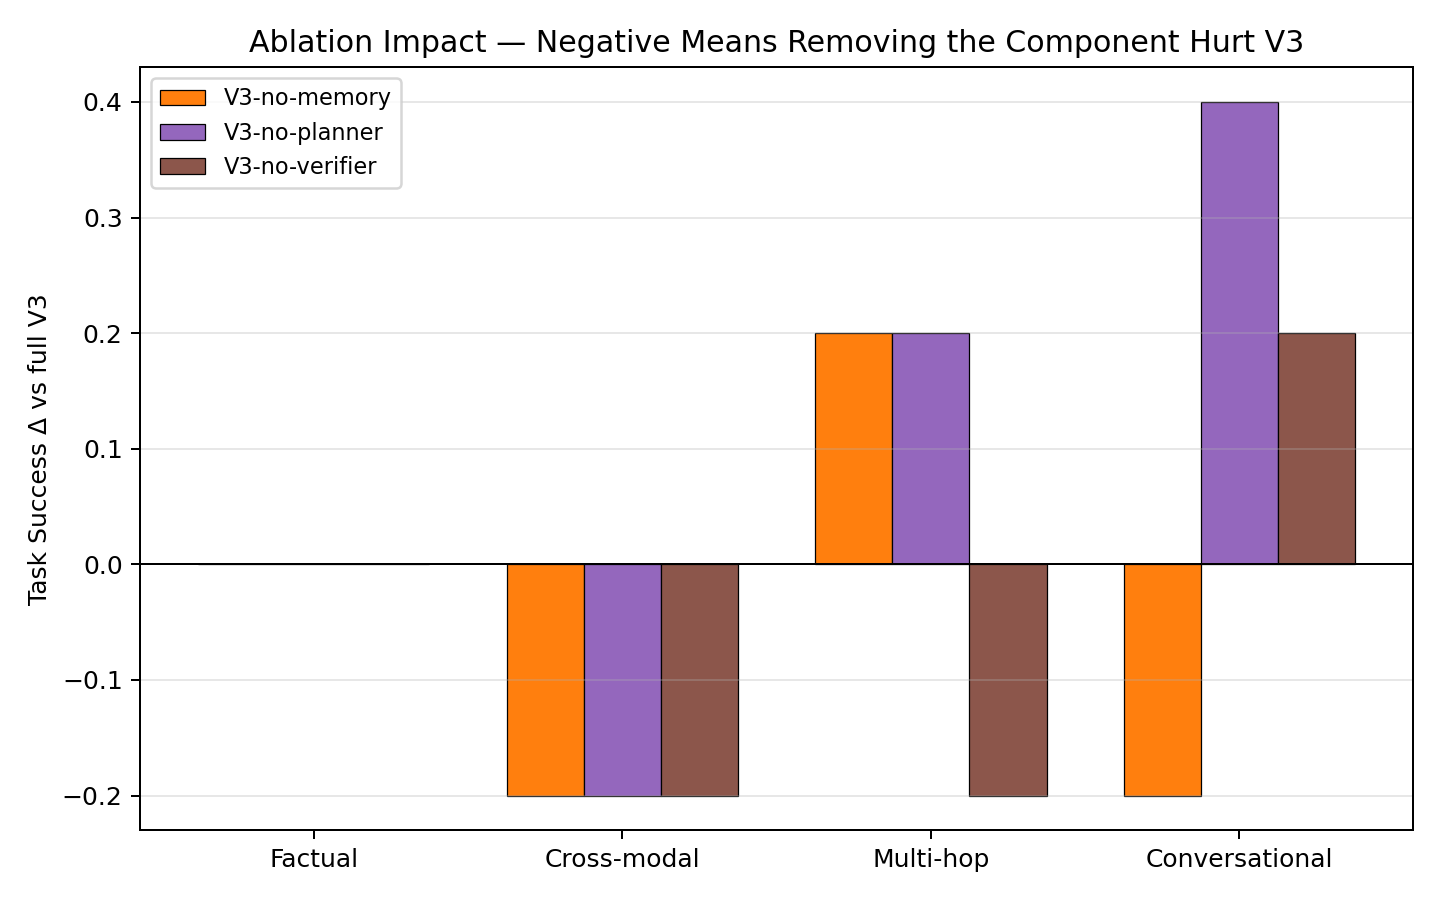
\includegraphics[width=\columnwidth]{eval/results/figures/ablation_delta.png}
\caption{Per-family task-success delta of each ablation versus full
V3. Negative bars mean removing the component hurt V3; positive bars
mean removing it \emph{helped}. The planner ablation is positive on
multi-hop and conversational --- structured planning was a net cost
on these families.}
\label{fig:ablation}
\end{figure}

Figure~\ref{fig:ablation} surfaces the most surprising result: the
\textsc{no-planner} ablation \emph{improved} task success on
conversational (\,$+$0.40) and multi-hop ($+$0.20). On four V3 failures
we manually inspected (QF3.1, QF3.3, QF4.4, QF4.5), the planner
produced either an empty plan or a plan whose filter step
over-constrained candidates from memory-derived facts; the verifier then
removed the remaining candidates and the generator was forced to
refuse (``\textit{I don't have a matching Cantonese dish in my
knowledge base}'') even though the matching recipe was in the KB.

The reactive (\texttt{bind\_tools}) path of V3-no-planner avoids this
trap by retrieving aggressively across multiple tool turns. Its cost
is correspondingly higher: an average of 15{,}955 tokens and 9.6 tool
calls per query (Table~\ref{tab:efficiency}) --- $\sim$3.6$\times$ the
tokens of full V3 and over 16$\times$ those of V1. It is a
Pareto-relevant configuration but not a Pareto winner.

\subsection{Failure mode breakdown}

\begin{table}[t]
\centering\small
\caption{Failure-mode counts per system ($N=20$ queries). Each failed
record is classified into exactly one of five categories.}
\label{tab:failures}
\begin{tabular}{lcccccr}
\toprule
System & Retr. & Q-grnd. & Grnd. & Reas. & Cite & \textbf{Total} \\
\midrule
V0              & 10 & 1 & 2 & 1 & 0 & 14 \\
V1              & 2  & 2 & 1 & 4 & 0 & 9  \\
V2              & 2  & 1 & 1 & 2 & 0 & 6  \\
V3 (full)       & 3  & 0 & 1 & 1 & 2 & 7  \\
V3-no-memory    & 4  & 0 & 3 & 1 & 0 & 8  \\
V3-no-planner   & 0  & 0 & 1 & 2 & 2 & 5  \\
V3-no-verifier  & 4  & 0 & 0 & 2 & 2 & 8  \\
\bottomrule
\end{tabular}
\end{table}

Table~\ref{tab:failures} shows the 5-class failure distribution. Three
patterns stand out: (i)~V0 is dominated by \textit{retrieval} failures
(10/14) --- it cannot retrieve, so it hallucinates or defers; (ii)~V1
and V2 shift toward \textit{reasoning} failures, indicating that
retrieval works but multi-hop aggregation breaks down (e.g. V1 on QF3.1
mentions only the winner without listing alternatives, failing
\textit{mentions-all-recipes}); (iii)~V3's failures concentrate in
\textit{retrieval} (empty candidates from over-constrained plans) and
\textit{citation} (recommends a recipe outside the constraint set in
multi-turn cases). V3-no-planner has the fewest failures overall (5)
and zero \textit{retrieval} failures, again pointing at the structured
plan as the brittle component.

\subsection{Cost--quality trade-off}

\begin{table}[t]
\centering\small
\caption{Efficiency averages across all 20 queries.}
\label{tab:efficiency}
\begin{tabular}{lrrr}
\toprule
System & Lat. (s) & Tokens & Tool calls \\
\midrule
V0              & 4.5  & 390     & 0.0 \\
V1              & 4.0  & 950     & 0.0 \\
V2              & 5.9  & 1{,}490 & 0.0 \\
V3 (full)       & 27.2 & 4{,}400 & 3.6 \\
V3-no-memory    & 17.9 & 3{,}070 & 2.8 \\
V3-no-planner   & 33.5 & 15{,}955 & 9.6 \\
V3-no-verifier  & 19.5 & 3{,}970 & 3.0 \\
\bottomrule
\end{tabular}
\end{table}

V0 is $\sim$11$\times$ cheaper than V3 and $\sim$41$\times$ cheaper than
V3-no-planner, while still attaining 0.6 on factual queries. The
report-worthy implication is that simple systems are
\emph{operationally rational} for simple queries; the marginal benefit
of agent complexity must be earned per query type.

% =====================================================================
\section{Discussion: When does complexity pay off?}
\label{sec:discussion}

Synthesising the result tables, Table~\ref{tab:guide} summarises the
configuration we would recommend per query family if cost were a
binding constraint --- which it normally is in production.

\begin{table}[t]
\centering\small
\caption{Recommended configuration per query family, based on
task success and token cost.}
\label{tab:guide}
\begin{tabular}{@{}ll>{\raggedright\arraybackslash}p{3.1cm}@{}}
\toprule
Family & Best system & Reason \\
\midrule
Factual        & \textbf{V1}              & retrieval suffices; $\sim$10$\times$ cheaper than V3 \\
Cross-modal    & \textbf{V3 / V2}         & V3 best on grounding; V2 if cost-sensitive \\
Multi-hop      & \textbf{V2 / V3-no-mem.} & both 0.60; V2 has half the latency \\
Conv.          & \textbf{V3-no-planner}   & only system $>$0.4; pay for it \\
\bottomrule
\end{tabular}
\end{table}

Two design implications follow. \emph{First}, the often-cited mantra
``retrieve-aggressively, filter-cautiously'' is supported: V3 fails
when its planner over-commits to a filter and the verifier prunes the
last candidate. \emph{Second}, the value of an agent depends on the
\emph{semantic ambiguity} of the query: factual look-ups need no
agent; ambiguous multi-turn requests benefit from broad reactive
retrieval. We see no single configuration that dominates the
Pareto frontier.

% =====================================================================
\section{Limitations and Future Work}
\label{sec:limits}

\textbf{Single LLM.} All seven systems share DeepSeek V4 Flash for
fair architectural comparison, but generalisation to GPT-4-class or
Claude-class models is not verified.
\textbf{KB scale.} 20 recipes is small; behaviour at $10^3$+ recipes
(where retrieval is the bottleneck rather than generation) may differ.
\textbf{Planner prompt.} Our V3 planner was not heavily tuned; a more
elaborated prompt with explicit ``prefer broad over empty plan'' rules
likely closes much of the no-planner gap. We report the unmodified
result because it preserves the integrity of the ablation.
\textbf{Metric edge cases.} On QF3.2, V3 attains task success $=1$ with
Recall@3 $=0$: the LLM's prior knowledge happened to produce the right
superlative without grounded retrieval. The same mechanism explains
V0's surprisingly high 0.60 on cross-modal queries --- the LLM knows
canonical visual properties (e.g.\ lasagna is layered) and gets credit
under our programmatic constraints, which reward correct mention
regardless of provenance. Both cases show task success and Recall@3
can decouple when surface heuristics align with gold answers.

% =====================================================================
\section{Conclusion}
\label{sec:conclusion}

Across 20 queries and 7 configurations, retrieval, multimodal fusion,
memory, and verification each carry positive marginal value, but
structured planning has \emph{negative} marginal benefit on the two
hardest query families. There is no single best agent; the best
configuration depends on the query type and the cost budget.
Rule-based programmatic evaluation made this conclusion auditable.

% =====================================================================
\begin{thebibliography}{9}
\bibitem{openclip}
G. Ilharco \emph{et al.},
``OpenCLIP,'' Zenodo, 2021. \texttt{https://github.com/mlfoundations/open\_clip}.

\bibitem{deepseek}
DeepSeek AI,
``DeepSeek V4 Preview API Documentation,'' 2026.
\texttt{https://api-docs.deepseek.com/}.

\bibitem{rag-triad}
TruEra,
``The RAG Triad: Context Relevance, Groundedness, Answer Relevance,''
TruLens Documentation, 2024.

\bibitem{langgraph}
LangChain,
``LangGraph: Build stateful, multi-actor applications with LLMs,'' 2024.
\texttt{https://langchain-ai.github.io/langgraph/}.

\bibitem{chromadb}
Chroma,
``Chroma: the AI-native open-source embedding database,'' 2024.
\texttt{https://www.trychroma.com/}.
\end{thebibliography}

\end{document}
